\chapter{Model} \label{chap:two}

% Parameter Table
\begin{table}
	\rowcolors{1}{}{lightgray}
	\centering
	\caption{Model parameters. \label{table:parameters}}
	\begin{tabular}{c p{.25in} p{4.5in}}
		$m$ & & Number of fibers \\
		$n_j$ & & Number of particles on the $j$th fiber, $1 \leq j \leq m$ \\
		$n_+$ & & Number of particles on the top substrate \\
		$n_-$ & & Number of particles on the bottom substrate \\
		$\delta_j$ & & Attachment point for the $j$th fiber on the bottom substrate, $1 \leq j \leq m$ \\
		$\ell$ & & Equilibrium distance for extensible springs \\
		$\ell_+$ & & Spacing between particles on the top substrate \\
		$\ell_-$ & & Spacing between particles on the bottom substrate \\
		$\beta$ & & Strength of torsional springs \\
		$\gamma$ & & Spring constant for extensible springs \\
		$\varepsilon$ & & Strength of vdW force between particles of fibers \\
		$\varepsilon_+$ & & Strength of vdW force between a particle on a fiber and a particle on the top substrate \\
		$\varepsilon_-$ & & Strength of vdW force between a particle on a fiber and a particle on the bottom substrate \\
		$\sigma$ & & Equilibrium distance between two particles for vdW \\
		$(\mu,\lambda)$ & & Load applied to the moving substrate \\
		$(x^{(+)}_0,y^{(+)}_0)$ & & Initial position for first particle on the top substrate \\
		$(x^{(-)}_0,y^{(-)}_0)$ & & Initial position for first particle on the bottom substrate
	\end{tabular}
\end{table}
	
	\begin{figure}
		\begin{center}
			\input{./fig/ch2/geometry.eps_tex}
		\end{center}		
		\caption{Geometry of a fiber pinned between the top and bottom substrates.
		\label{fig:Geometry}}
	\end{figure}		
	
\section{Geometry}

   We consider a collection of particles linked into a chain that we call a fiber. Each fiber is connected to a stationary horizontal (bottom) substrate at some fixed position. We also consider a (top) substrate that is always parallel to the bottom substrate and that only translates. There are two artificial particles associated with each fiber, one at the connection (or attachment) point with the bottom substrate and an additional particle placed at any point on a half circle below the bottom substrate of radius one. We call the particle at the attachment point the attachment particle, and the other particle below it the floating particle (see Figure~\ref{fig:Geometry}). The system consists of $m$ fibers, with $n_j$ particles for the $j$th fiber, a top substrate with $n_+$ particles, and a bottom substrate with $n_-$ particles.
	
We denote the position vector of the $i$th particle on the $j$th fiber by
\begin{equation}
	\textbf{r}_i^{(j)} = (x_i^{(j)},y_i^{(j)})
\end{equation}
where $1 \leq j \leq m$ and $1 \leq i \leq n_j$. We also define the following vectors for convenience,
\begin{equation}
	\Delta \textbf{r}_i^{(j)} = \textbf{r}_i^{(j)} - \textbf{r}_{i-1}^{(j)}.
\end{equation}
The two artificial particles are denoted as follows,
\begin{equation}
	\textbf{r}_0^{(j)} = (x_0^{(j)},y_0^{(j)}) = (\delta_j,0)
\end{equation}
for the attachment particle and
\begin{equation}
	\textbf{r}_{-1}^{(j)} = (x_{-1}^{(j)},y_{-1}^{(j)}).
\end{equation}
for the floating particle.

	The chain of particles is a discrete analog to a CNT (see Figure~\ref{subfig:NanotubeParticle}). Indeed, the vectors $\Delta \textbf{r}_i^{(j)}$ conceptually represent the interparticle bonds in this geometry. However, this approach is sufficiently generic to describe other fiber structures and we do not limit our discussion to this motivation.
	
	The bottom substrate as described before is attached to every fiber at the attachment particle. We define two position vectors,
\begin{eqnarray}
	\textbf{r}_0^{(+)} = (x_0^{(+)},y_0^{(+)}) & \\
	\textbf{r}_i^{(+)} = (x_0^{(+)} + i\ell_+,y_0^{(+)}), & 0 < i < n_+
\end{eqnarray}
for the top substrate and,
\begin{eqnarray}
	\textbf{r}_0^{(-)} = (x_0^{(-)},y_0^{(-)}) & \\
	\textbf{r}_i^{(+)} = (x_0^{(+)} + i\ell_-,y_0^{(+)}), & 0 < i < n_-
\end{eqnarray} 
for the bottom substrate. Since both substrates are rigid, the bottom substrate is stationary, and the top substrate is only allowed to translate, the positions of all particles on each substrate can be respectively specified by identifying the position of a single particle. Both particles are decided as initial conditions together with the initial positions of every particle on each fiber. The rest of the particles on either substrate are defined by a parameter for the total number of particles, and an interval spacing, $\ell_+$ and $\ell_-$.

\section{Energy}

	We want a fiber to be in equilibrium when all particles are collinear and each particle is a fixed distance $\ell$ away from its neighbors. In order to enforce this equilibrium configuration we incorporate two types of springs into the model: an extensible spring and a torsional spring.

\subsection{Extensible spring}

	The extensible spring is described by the standard Hooke's law with spring constant $\gamma$ and is meant to keep any two adjacent particles on a fiber a fixed distance $\ell$ apart. The energy for all extensible springs in the system is then
\begin{equation}
	E_e = \gamma \sum_{j=1}^m \sum_{i=1}^{n_j} \left[ \left( \|\Delta \textbf{r}_i^{(j)} \| - \ell \right)^2 \right].
\end{equation}
Note that there is no spring between the floating particle and the attachment particle, but there is a spring between the attachment particle and the $\textbf{r}_0^{(j)}$ particle on the $j$th fiber. Both the attachment particle and the floating particle are introduced into the system to model the connection between the fiber and the bottom substrate. The spring between the attachment particle, $\textbf{r}_0^{(j)}$, and the particle, $\textbf{r}_1^{(j)}$, enforces attachment of the $j$th fiber.

	\begin{figure}
		\begin{center}
			\input{./fig/ch2/torsionenergy.eps_tex}
		\end{center}		
		\caption{Two vectors $\textbf{a}$ and $\textbf{b}$, representing links between three particles and a corresponding angle measured against the positive $x$-axis centered at each tail point. The bending energy will be minimized when the difference in angle is zero, or the particles are collinear.
		\label{fig:BendingEnergy}}
	\end{figure}	

\subsection{Torsional spring}

	The extensible springs alone are not sufficient to describe the kind of equilibrium we seek, so we introduce an energy penalty for bending, when the adjacent particles are not collinear (see Figure~\ref{fig:BendingEnergy}). We choose the expression,
\begin{equation}
	e_b = 2\beta \tan^2 \left( \frac{\Delta \theta}{2} \right),
\end{equation}
to represent the energy of a torsional spring at the junction between two bonds. Here $\beta$ is the strength of the spring. Notice this energy diverges as $\Delta \theta \to \pm180$\textdegree to guarantee that the bonds to do fold onto themselves. The geometry of the system is described in terms of particles, not angles, hence we rewrite the energy in terms of position vectors,
\begin{equation}
	E_b = 2\beta \sum_{j=1}^m \sum_{i=1}^{n_j} \left[ \frac{\|\Delta \textbf{r}_i^{(j)} \| \|\Delta \textbf{r}_{i-1}^{(j)} \| - \Delta \textbf{r}_i^{(j)} \cdot \Delta \textbf{r}_{i-1}^{(j)}}{\|\Delta \textbf{r}_i^{(j)} \| \|\Delta \textbf{r}_{i-1}^{(j)} \| + \Delta \textbf{r}_i^{(j)} \cdot \Delta \textbf{r}_{i-1}^{(j)}} \right].
\end{equation}

	This energy incorporates every contiguous set of three particles, including the two artificial particles. With the incorporation of the angle between the artificial particles and the particle, $\textbf{r}_0^{(j)}$, the optimal angle of the fiber with respect to the substrate can be tuned according to the placement of the floating particle. For example, if the angle between the artificial bond connecting the floating particle to the attachment particle, and the first bond connecting the attachment particle to particle $\textbf{r}_0^{(j)}$ is $90$\textdegree, then the entire fiber will want to be upright. If the equilibrium attachment angle is $45$\textdegree, then the entire fiber will want be slanted at $45$\textdegree,~etc. 

   The system of extensible and torsional springs is sufficient to model the equilibrium behavior of a system of isolated noninteracting fibers. However, we are still motivated by a nanoscale setting, namely that of CNTs. We introduce a particle-particle interaction to model the kinds of molecular forces we would expect on a nanoscale.

\subsection{van der Waals interactions}	

	\begin{figure*}[t!]
		\centering
		\begin{subfigure}[t]{.5\textwidth}
			\centering
			\includegraphics[scale=.5]{./fig/ch2/lj_e.eps}
			\caption{Lennard-Jones energy, well depth is $\varepsilon$, minimized at $\sigma$. \label{subfig:LJEnergy}}
		\end{subfigure}%
		~
		\begin{subfigure}[t]{.5\textwidth}
			\centering
			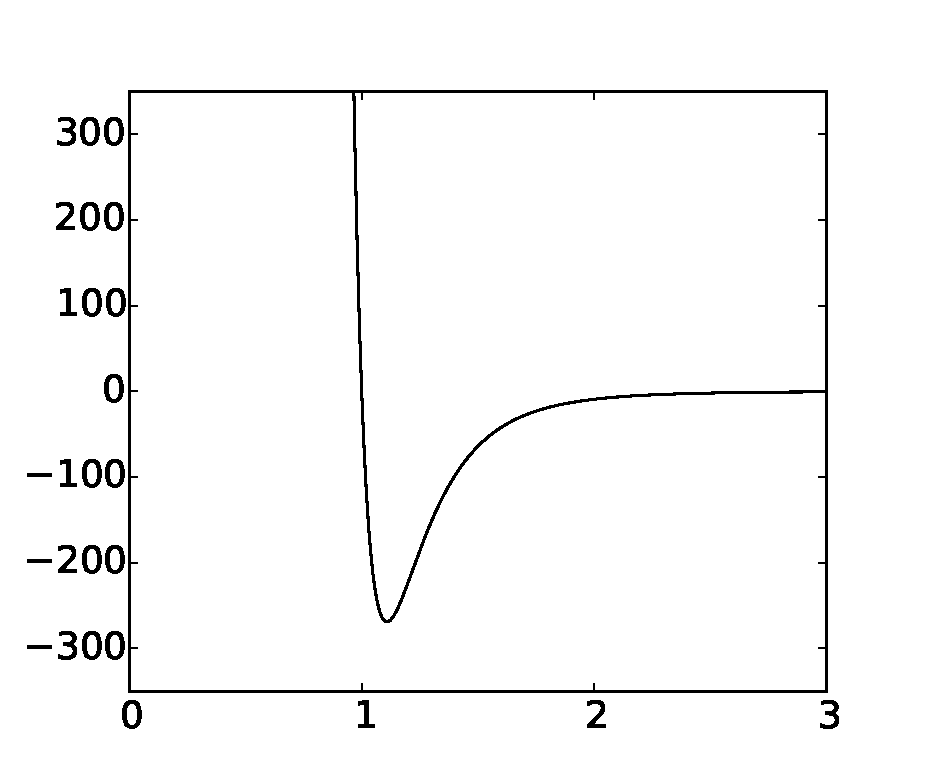
\includegraphics[scale=.5]{./fig/ch2/lj_f.eps}
			\caption{Lennard-Jones force. \label{subfig:LJForce}}
		\end{subfigure}		
		\caption{Lennard-Jones 12-6 potential and force with $\sigma = 1$ and $\varepsilon = 100$.\label{fig:LJ}}	
	\end{figure*}

   Van der Waals' (vdW) interaction are used to describe the sum of attractive and repulsive forces of atomic structures that are not accounted for by their covalent bonds. In a CNT setting we consider the extensible spring already described as an abstraction of covalent bonding of carbon atoms but we have yet to account for any vdW interaction. We use a truncated Lennard-Jones 12-6 potential to represent the vdW interactions between each particle in the model. The Lennard-Jones potential is parameterized by the strength of the interaction, $\varepsilon$, and the equilibrium distance between two interacting particles, $\sigma$ (see Figure~\ref{fig:LJ}). An exception is made for particles with an extensible spring between them. Stated precisely, there is vdW interaction between every particle and every other particle except if the two particles are adjacent on the same fiber.
	
The standard Lennard-Jones potential,
\begin{equation}
	U(x; \varepsilon, \sigma) = \varepsilon \left[ \left( \frac{\sigma}{x} \right)^{12} - 2 \left( \frac{\sigma}{x} \right)^6 \right],
\end{equation}

	\begin{figure*}[t!]
		\centering
		\begin{subfigure}[t]{.5\textwidth}
			\centering
			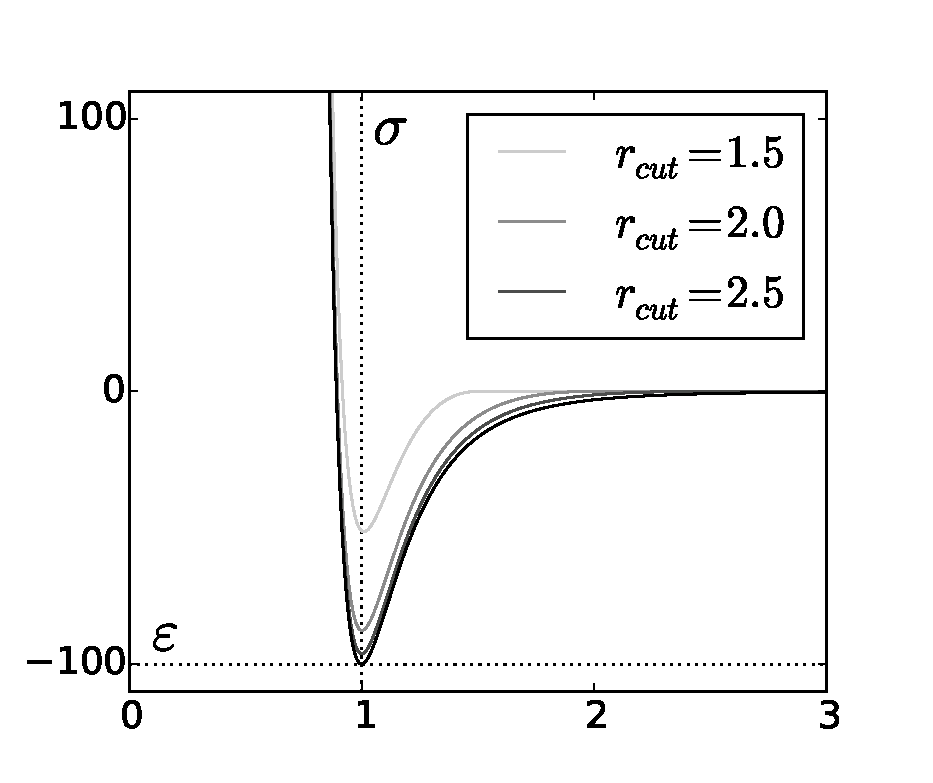
\includegraphics[scale=.5]{./fig/ch2/ljc_e.eps}
			\caption{Truncated Lennard-Jones energy. \label{subfig:LJTEnergy}}
		\end{subfigure}%
		~
		\begin{subfigure}[t]{.5\textwidth}
			\centering
			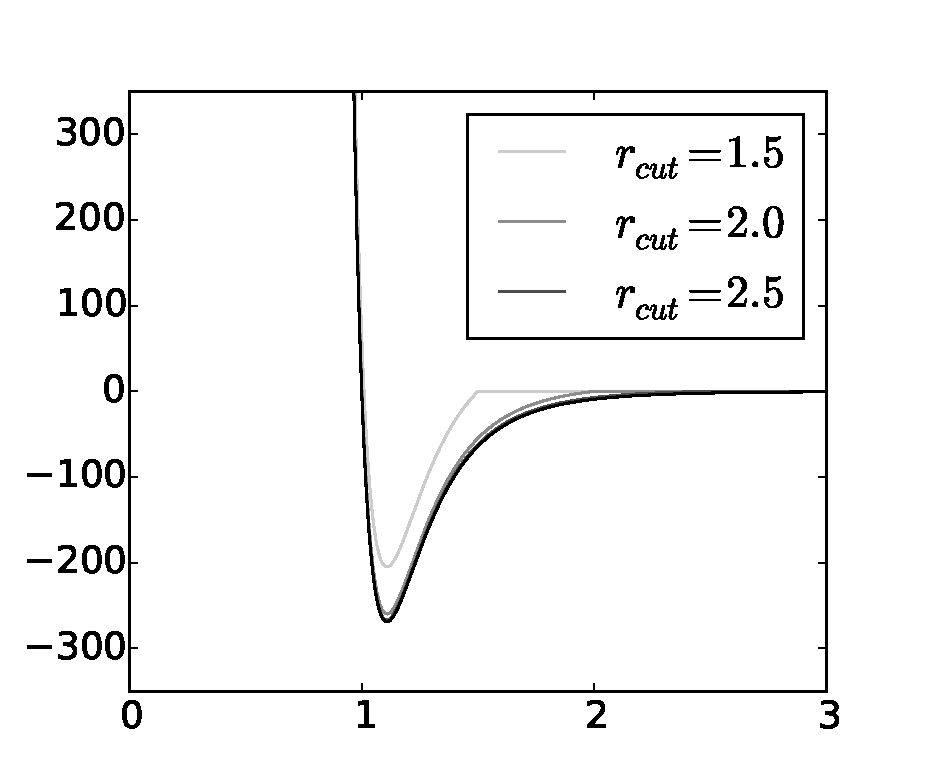
\includegraphics[scale=.5]{./fig/ch2/ljc_f.eps}
			\caption{Truncated Lennard-Jones force. \label{subfig:LJTForce}}
		\end{subfigure}		
		\caption{Lennard-Jones energy and force are in black in the respective figures as reference.\label{fig:LJT}}	
	\end{figure*}	

\noindent	
asymptotically approaches zero as $x$ approaches infinity. This makes Lennard-Jones a short range potential and, more importantly, makes interactions at long distances negligible. We can truncate (or cut) the potential at some radius $r_c$. However, this introduces a discontinuity in the potential, so in order to repair both the potential and it's derivative, we use the following modification,
\begin{equation}
	U_c(x; \varepsilon, \sigma) = \left\{ 
		\begin{array}{lr}
			U(x; \varepsilon, \sigma) - U(r_c; \varepsilon, \sigma) - \frac{dU}{dx}\bigg|_{x = r_c}(x - r_c), & x \leq r_c\\
			0, & x > r_c
		\end{array}
		\right. 
\end{equation}

	The sequence of truncated Lennard-Jones potentials converges to the Lennard-Jones potential as $r_c \to \infty$ and the truncated Lennard-Jones potentials share the same asymptotic behavior (see Figure~\ref{fig:LJT}). This truncation technique is referred to as shifted forces, it is commonly used to conserve energy in the potential and avoid potential artifacts with a model. The discontinuous truncation is also used but can cause larger discrepancies in energy particularly with very long simulations. Although this method alters the potential everywhere the accuracy with respect to the true potential has been observed in molecular dynamics simulations as better than the discontinuous truncation \cite{Toxvaerd2011}.
	
  Time dependent simulations leading to equilibrium for large systems can require long time intervals, so to avoid artifacts in the geometry we use the continuous variation of the truncated Lennard-Jones potential. Moreover, we pick a conservative cutoff selection of $r_c = 8$ in all simulations to further ensure accuracy of equilibrium configurations.

	In order to represent concisely the set of particles that a given particle is interacting with, we define the set
\begin{equation}
	P(j,i) = \{ (h,k)|j \neq h \vee k \neq i \pm 1, 1 \leq h \leq m, 1 \leq k \leq n_h \},
\end{equation}
which contains every particle that the $i$th particle on the $j$th fiber interacts with via the truncated 12-6 potential. Now we can express the vdW energy for the system,
\begin{multline}
	E_v = \sum_{j=1}^m \sum_{i=1}^{n_j} \bigg[ \sum_{(h,k) \in P(j,i)} U_c \left( \| \textbf{r}_i^{(j)} - \textbf{r}_k^{(h)} \|; \varepsilon, \sigma \right) \\ + \sum_{k=1}^{n_-} U_c \left( \| \textbf{r}_i^{(j)} - \textbf{r}_k^{(-)} \|; \varepsilon_-, \sigma \right) + \sum_{k=1}^{n_+} U_c \left( \| \textbf{r}_i^{(j)} - \textbf{r}_k^{(+)} \|; \varepsilon_+, \sigma \right) \bigg].
\end{multline}
It is not the case that the interaction strength is the same for each potential. There are different strengths for fiber to fiber, fiber to top substrate, and fiber to bottom substrate interactions.

% van der Waals lower substrate pressure
%\begin{equation}
%	E_p = \sum_{j=1}^m \sum_{i=1}^{en_j} U_p \left( y_i^{(j)} \right)
%\end{equation}

\subsection{Total energy and dynamics}

With both springs and vdW interaction the system of fibers and the bottom substrate is complete. What is left is the rigid motion of the top substrate. We apply a load with a vertical component, $\lambda$, and horizontal component, $\mu$, to the top substrate. Recall, that the top substrate is only allowed to undergo translational motion parallel to the bottom substrate.

With all interactions in the system defined, the total energy of the system is

% Total energy
\begin{equation}
	E = E_b + E_e + E_v + \lambda x_0^{(+)} - \mu y_0^{(+)}.
\end{equation}
The model for the system includes two springs, the extensible and torsional springs, the vdW interaction, and the rigid motion of the top substrate. Note that the signs for $\lambda$ and $\mu$ are selected so that positive vertical load is pointing downward, while positive horizontal load points to the right.

Using Newton's second law with a damping term we have,

\begin{equation}
	M\frac{d^2\textbf{r}_i^{(j)}}{dt^2} + \frac{d\textbf{r}_i^{(j)}}{dt} = -\nabla_{\textbf{r}_i^{(j)}}E,
\end{equation}
for the $i$th particle on the $j$th fiber, where $M$ is the mass of the particle. Here we assume the particles are massless so that the acceleration is negligible, that is

\begin{equation} \label{eqn:system}
	 \frac{d\textbf{r}_i^{(j)}}{dt} = -\nabla_{\textbf{r}_i^{(j)}}E,\ \ \ 1 \leq j \leq m,\  1 \leq i \leq n_j.
\end{equation}
The evolution of the physical system governed by \eqref{eqn:system} drives the energy towards a minimum.

\section{Implementation}

   In this section we discuss the simulation procedure utilized in Chapter~\ref{chap:three} and Chapter~\ref{chap:four} and presented in Appendix~\ref{ap:c}. We omit details of standard library algorithms and focus instead on details on nonstandard implementations of algorithms we employ.

   The choice of a truncated Lennard-Jones potential allows for an optimization that improves the average number of interactions that need to be computed. The optimization in this work uses the Verlet neighbor list method. This method improves computation at every time step from O(n^2) to O(n). 
   
   TODO: just describe Verlet neighbor list method in detail
   
   The saving comes from the fact that if you have to update the list then you still have to do O(n^2) interactions, so you do an O(n) check every time step and save on when it doesn't have to be updated.
   
   
   The trade off becomes an $\mathcal{O}(n)$ algorithm at each time step to determine if the list needs to be updated. Each time step the two largest displacements of unique particles are computed. If the sum of these displacements is larger than the buffer distance of the Verlet neighbor list then the list must be updated. The buffer zone in our case is the distance from our cutoff, $r_c = 8$, and a second cutoff, $r_{max} = 12$. For all simulations discussed here we have a buffer radius of $4$. Verlet neighbor lists are not the only manner of implementing the optimization and the reader may be interested in other solutions, such as cell lists.

   Equilibrium configurations are hard to decide on because we don't have infinite computation time to make sure nothing changes numerically. To ensure that the algorithm eventually stops we need an equilibrium criterion that when satisfied declares the system in equilibrium. In our case the equilibrium criterion is relative. That is, we take the norm distance between the current state vector and the prior state vector of the system. If this distance is less than a tolerance, $10^{-8}$, we mark the system as in equilibrium. We require that this condition is satisfied for ten consecutive time steps as the practical stopping criterion.
   
   Another stopping criterion is if the velocity of the top substrate is within $10^{-8}$ of a prescribed maximum velocity, $\frac{\sqrt{\lambda^2 + \mu^2}}{\Delta t}$, then we can stop the simulation early. As before, this must hold for ten time steps before the simulation ends. We discuss this stopping criterion in greater detail in Section~\ref{ch:detachment}.
   
   The numerical procedure was implemented in both MATLAB \cite{MATLAB2010} (Appendix~\ref{ap:b}) and C/C++ (Appendix~\ref{ap:c}). The results presented in this thesis were obtained using the C/C++ version. However, the MATLAB version was run for some test cases to verify the compare against the C/C++ version. The software package SUNDIALS (CVODE \cite{sundials}) was used to evolve the system at each time step. All figures were generated using MatPlotLib \cite{Hunter2007} with Python (Appendix~\ref{ap:a}) and Inkscape.
